\documentclass{article}
\usepackage[utf8]{inputenc}
\usepackage{tikz, pgfplots}
\usetikzlibrary{positioning}
\begin{document}

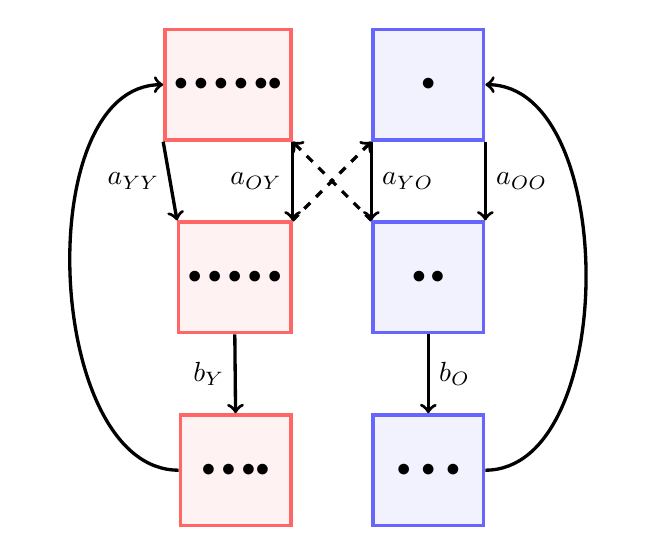
\begin{tikzpicture}[
youngnode/.style={rectangle, draw=red!60, fill=red!5, very thick, minimum size=40},
oldnode/.style={rectangle, draw=blue!60, fill=blue!5, very thick, minimum size=40},
]
%Nodes
\node[oldnode]        (DF1)                            { $\bullet$};
\node[oldnode]        (DF2)       [below=of DF1]      { $\bullet\,\bullet$};
\node[oldnode]        (DF3)       [below=of DF2]      { $\bullet\,\bullet\,\bullet$};

\node[youngnode]      (DF6)        [left=of DF1]      {$\bullet\bullet\bullet\bullet\bullet\bullet$ };
\node[youngnode]      (DF5)        [left=of DF2]      {$\bullet\bullet \bullet \bullet\bullet$};
\node[youngnode]      (DF4)        [left=of DF3]      { $\bullet\bullet \bullet\bullet$};

%Lines
\draw[->, very thick] (DF1.south east)  to node[right] {$a_{OO}$} (DF2.north east);
\draw[->, very thick] (DF2.south)  to node[right] {$b_O$} (DF3.north);
\draw[->, very thick] (DF3.east)  .. controls  +(right:17mm) and +(right:17mm)   .. (DF1.east);

\draw[->, very thick] (DF6.south west)  to node[left] {$a_{YY}$} (DF5.north west);
\draw[->, very thick] (DF5.south)  to node[left] {$b_Y$} (DF4.north);
\draw[->, very thick] (DF4.west) .. controls  +(left:17mm) and +(left:17mm)   .. (DF6.west);

\draw[dashed,->, very thick] (DF2.north west)  to  (DF6.south east);
\draw[->, very thick] (DF6.south east)  to node[left] {$a_{OY}$} (DF5.north east);

\draw[->, very thick] (DF1.south west)  to node[right] {$a_{YO}$} (DF2.north west);
\draw[dashed,->, very thick] (DF5.north east)  to  (DF1.south west);
\end{tikzpicture}

\end{document}